\outline{1}{Variability of Movements in Joint Space Predicts Learning and Recovery	in Exoskeleton Training Post-Stroke}
\chapter{Variability of Movements in Joint Space Predicts Learning and Recovery	in Exoskeleton Training Post-Stroke}
\label{cha:armeospring}


\outline{2}{Introduction}
\section{Introduction}

Initial behavioral changes post-stroke largely result from “spontaneous recovery”, which is greatest in the first month and continues for $ \sim $6 months \cite{Duncan1992, Duncan2000}. 
Spontaneous recovery involves reduction in lesion edema, ischemic penumbra, and brain reorganization \cite{Bains2014, Murphy2009}. 
Motor training consisting of thousands of movements over weeks is thought to influences speed and level of recovery via slow re-organization of surviving neural networks \cite{Nudo1996, Pavlides1993, Wolf2006, Lincoln1996}. 
Evidence points that UE training improves reaching movements’ speed, smoothness, and range(e.g. \cite{Anton1996}).
As a result, a large number of studies, and devices, have been developed to retrain arm movements post-stroke. 

However, during robotic or mechanized training, the environment is “perturbed” compared to movements in daily activities. 
For instance, during training with the MIT-Manus robot, the movements are in the horizontal plane, with the hand supported by the robot handle. 
As such, gravity has a reduced effect during movements. 
Similarly, in the ARMEO Spring exoskeletons used in the present study, gravity is compensated via adjustable springs in both the proximal and distal arm segments.
Accordingly, the participants are making movements in a new force field. 
Because of sensori-motor adaptation to these force fields, it is unclear what are the causes the observed improvements: motor learning due to the new environment, recovery, or both. 

Here, we study recovery of arm movement in 50 individuals in the sub-acute phase post-stroke during 20 sessions of training with the ARMEO spring exoskeleton over 4 weeks.
Our first objective is to dissociate the effects of motor learning, presumably occurring at a relatively fast time scale, from recovery, presumably at a lower time scales.  
For this purpose, we use mixed-effect double exponentials models fitted to end-effector kinematic data. 
The double exponentials help us to dissociate between a faster and a slower phase of improvements. 
The mixed effects allow us to take into account the large variability in initial performance and changes in performance within the heterogeneous stroke subjects.

Our second objective is to identify predictors of such recovery and learning. 
A possible candidate for the modulation of recovery is the pattern of joint movements. 
Stroke survivors usually display atypical upper extremity movement patterns, referred to as abnormal ``synergies" \cite{Brunnstroem1970}. 
Because of the redundancy in the number of arm joints, many different combinations of joint angles can create the same hand position and orientation. 
Thus, improvements in reaching performance (measured in end-effector space) can result either from compensatory adaptation, in which the patient uses alternate degrees of freedom and/or muscles to complete the task, or from true recovery of normative movement patterns \cite{Roby-Brami2003}. 
For example, to reach a target, patients often generate exaggerated forward trunk movements \cite{Roby-Brami2003}, or exaggerated shoulder elevation \cite{Steenbergen2000}.  
Such compensation may ultimately impede recovery however \cite{Roby-Brami2003}; contrarily, it has been shown that reduction of compensatory trunk movement for instance decreased long-term impairments in the arm \cite{Michaelsen2006}. 
Here, our hypothesis is that individuals post-stroke who show patterns of joint movements similar to non-disabled subject will recover faster than those who exhibit dissimilar, compensatory, movements.
For this, we use Principal Component Analysis (PCA) to quantify joint synergies \cite{Kordelaar2012} in both stroke and non-disabled individuals.

A possible candidate for the modulation of motor learning is movement variability in the null space of the joint angles. 
It has been proposed that movement variability in non-disabled individuals can influence motor learning. 
The redundancy of human arm kinematics dictates that there must be task-irrelevant variability, that is, variability that does not affect endpoint trajectories, in the joint space \cite{Scholz1999}. 
Recently, \cite{Singh2016} shows that redundancy in joint space is exploited by non-disabled individuals to facilitate learning. 
Here, our hypothesis is that task-irrelevant variability during training with the redundant ARMEO Spring will modulate motor learning in individuals post-stroke.

This work is in collaboration with Denis Mottet\footnote{\label{montepellier}\textit{STAPS, Universite de Montepellier and Euromov, Montpellier, France}}, Isabelle Laffont\footnotemark[\ref{montepellier}], Dave Reinkensmeyer\footnote{\textit{Department of Mechanical and Aerospace Engineering, University of California, Irvine, USA}}, Nicolas Schweighofer\footnote{Biokinesiology and Physical Therapy, University of Southern California, Los Angeles, USA} and Olivier Remy Neris\footnote{Universite de Bretagne Occidentale, Brest, France}. 

\outline{2}{Methods}
\section{Methods}

\subsection{Participants}

Arm movements kinematics was collected using ARMEO Spring devices in a sub-cohort of participants included in the experimental group of the REM-AVC clinical trial (NCT01383512), a 22-center medico-economic study of mechanized arm therapy post-stroke. 
This 5-year 20-center RCT aims at evaluating the medico-economic benefits in post-acute stroke of 4 weeks of standard care and motor arm therapy with ARMEO Spring vs. standard care and self-rehabilitation. 
Main inclusion criteria are: 1) a stroke between 4 to 12 weeks prior to enrollment, 2) ability to move the arm with UEFM score from 10 to 40. 

Kinematic and clinical data of 53 participants were available for the present study (30 males, 19 females, 4 gender not available; 59.3 $\pm$ 13.9 years old (All reported values are mean $\pm$ standard deviation), UEFM at baseline 24.7 $\pm$ 9.1, time since stroke 8.0 $\pm$ 3.0 weeks). 
The participants were scheduled to receive 4 weeks of ARMEO training, 5 days/week, twice/day. 
Baseline UEFM was measured in the week before training and again in the week following training by physical or occupational therapists who were all trained to administering the UEFM. 
To quantify normative performance 11 non-disabled individuals (4 females, 23.5 $\pm$ 2.0 years) performed 10 training sessions for 5 days. 
Training sessions lasted about 30 minutes each, and included a vertical pointing tests at the start and end of each session (thus, there were 4 tests/day). 
The data analyzed here is the end-effector trajectory and joint rotation data in these tests.

\begin{table}[b]
\footnotesize
	\begin{tabular}{|c|c|c|c|c|c|c|c|}
		\hline
		Group & No. & Age & Affected Side & Gender & UEFM & Post Stroke Days & Prescribed \\
		&&&&&  pre to post & & No. of Tests		\\
		\hline
		\multirow{2}{*}{Stroke} & \multirow{2}{*}{53} & \multirow{2}{*}{59$\pm$14} & 29L, 24R, & 19F, 30M, & 25$\pm$9 to & 56$\pm$21 & 80 in 4 weeks \\ 
		&&& 4 Unknown & 4 Unknown & 39$\pm$14 && \\
		\hline
		Control & 11 & 23$\pm$2 & - & 4F, 7M & - & - & 20 in 1 weeks \\
		\hline
	\end{tabular}
	\caption{Participants information}
	\label{tab:demog}
\end{table}

\subsection{The ARMEO Spring Device}

The ARMEO Spring exoskeleton\footnote{https://www.hocoma.com/us/solutions/armeo-spring/} has 6 degrees of freedom, summarized in Table \ref{tab:devicedof} and Figure \ref{fig:1setupschedule}B. 
It has two adjustable gravity-compensating springs, at upper arm and the forearm respectively. 
Lengths of the segment are also adjustable to adapt to user’s arm length. 
There are no motors at any joints; user must move actively to control the exoskeleton. 
The arm is attached to the exoskeleton via Velcro straps; movement of the user’s trunk is mildly constrained by a Velcro strap at the upper arm.

The device records all joint angles, and calculates in real time the end effector location through a forward kinematics model of the exoskeleton. 
The end effector location then is used to control a cursor on a screen, displayed vertically in front of the user, with which the vertical test and other different games are played. 
All joint angles and end effector locations are recorded. As seen in Table \ref{tab:devicedof}, most ARMEO angles do not correspond to anatomical angles: in particular, anatomical shoulder rotation and elbow flexion/extension are given by a combination of ARMEO upper arm and elbow joints movements. 

%\textbf{Device.}
%Our robot-aided rehabilitation uses Armeo@Spring exoskeleton from Hocoma\footnote{https://www.hocoma.com/us/} for therapy training. 
%Shown in figure \ref{fig:1setupschedule}, the exoskeleton has 6 degrees of freedom, summarized in table \ref{tab:devicedof} and Figure \ref{fig:1setupschedule}B. 
%It is attached to the arm by two or three velcro straps. 
%The exoskeleton has two springs equipped, at the upper arm and the forearm respectively. 
%The springs can be adjusted to compensate the gravity force of the arm. 
%Lengths of the exoskeleton are also adjustable to adapt to user's arm length.
%There are no motors at any joints; user has to move actively to control the exoskeleton. 
%User's trunk is mildly constrained by the velcro strap at the upper arm.

\begin{table}
	\begin{tabular}{|c|c|c|c|}
		\hline
		Joint No. & Angle Name & Anatomical Counterpart & Direction \\
		\hline
		1(a) & Inner Shoulder Horizontal & Shoulder Horizontal & Left/Right \\
		& Angle (SH)& Ab-/Adduction &\\ \hline
		1(b) & Outer Shoulder Horizontal & Shoulder Horizontal & Left/Right \\
		& Angle (SH)& Ab-/Adduction &\\ \hline
		2 & Shoulder Elevation Angle (SE) & Shoulder Flex-/Extension & Up/Down \\ \hline
		3 & Elbow Angle (EL) & - & Left/Right \\ \hline
		4 & Forearm Angle (FA) & - & Up/Down \\ \hline
		5 & Pro-/Supination Angle & Pro-/Supination & - \\  \hline
		6 & Wrist Flex-/Extension Angle & Wrist Flex-/Extension & - \\
		\hline
	\end{tabular}
	\caption{Degrees of freedom of ArmeoSpring exoskeleton.}
	\label{tab:devicedof}
\end{table}

\subsection{Training and Testing}
Participants in the stroke group received two training sessions, one in the morning and one in the afternoon per day, every weekday for four consecutive weeks (Figure \ref{fig:1setupschedule}C). 
Participants in the control group received two training sessions (morning and afternoon) for five consecutive days in a week. 
One training session lasted between 20 and 30 minutes, and consisted of a number of different games provided by Hocoma, the ARMEO Company.
The therapists and patients selected the games in each session.  

A vertical ladybug-pointing test (provided by Hocoma\footnote{https://www.hocoma.com/us/}) was scheduled at the beginning and the end of each training session. 
This test was two-dimensional; the movement along the dimension perpendicular to the frontal (coronal) plane was ignored. 
In this test, the user was instructed to catch ladybug targets that appeared sequentially on the screen. 
The sequence of target locations appeared random to the subject but was fixed in each test. 
To catch the ladybug, the user moved the cursor to its location. 
The user had limited time to catch the ladybug ($<$ 10 seconds). 
After a ladybug was caught, or the time limit was reached, the ladybug disappeared and the next ladybug appeared at a new location. 
There were four possible difficulty levels for the test; difficulty was modulated both by the number of targets and by the workspace size; from easy to difficult: 12 targets, 24 $ \times $ 16 cm (horizontal $ \times $ vertical);  20 targets, 36 $ \times $ 27 cm ; 32 targets, 45 $ \times $ 36 cm and 48 targets, 63 $ \times $ 45 cm. In the stroke group, test difficulty was adjusted by the therapist based on performance. 
In the control group, difficulty was set to the highest level. 


\begin{figure}
	\centering
	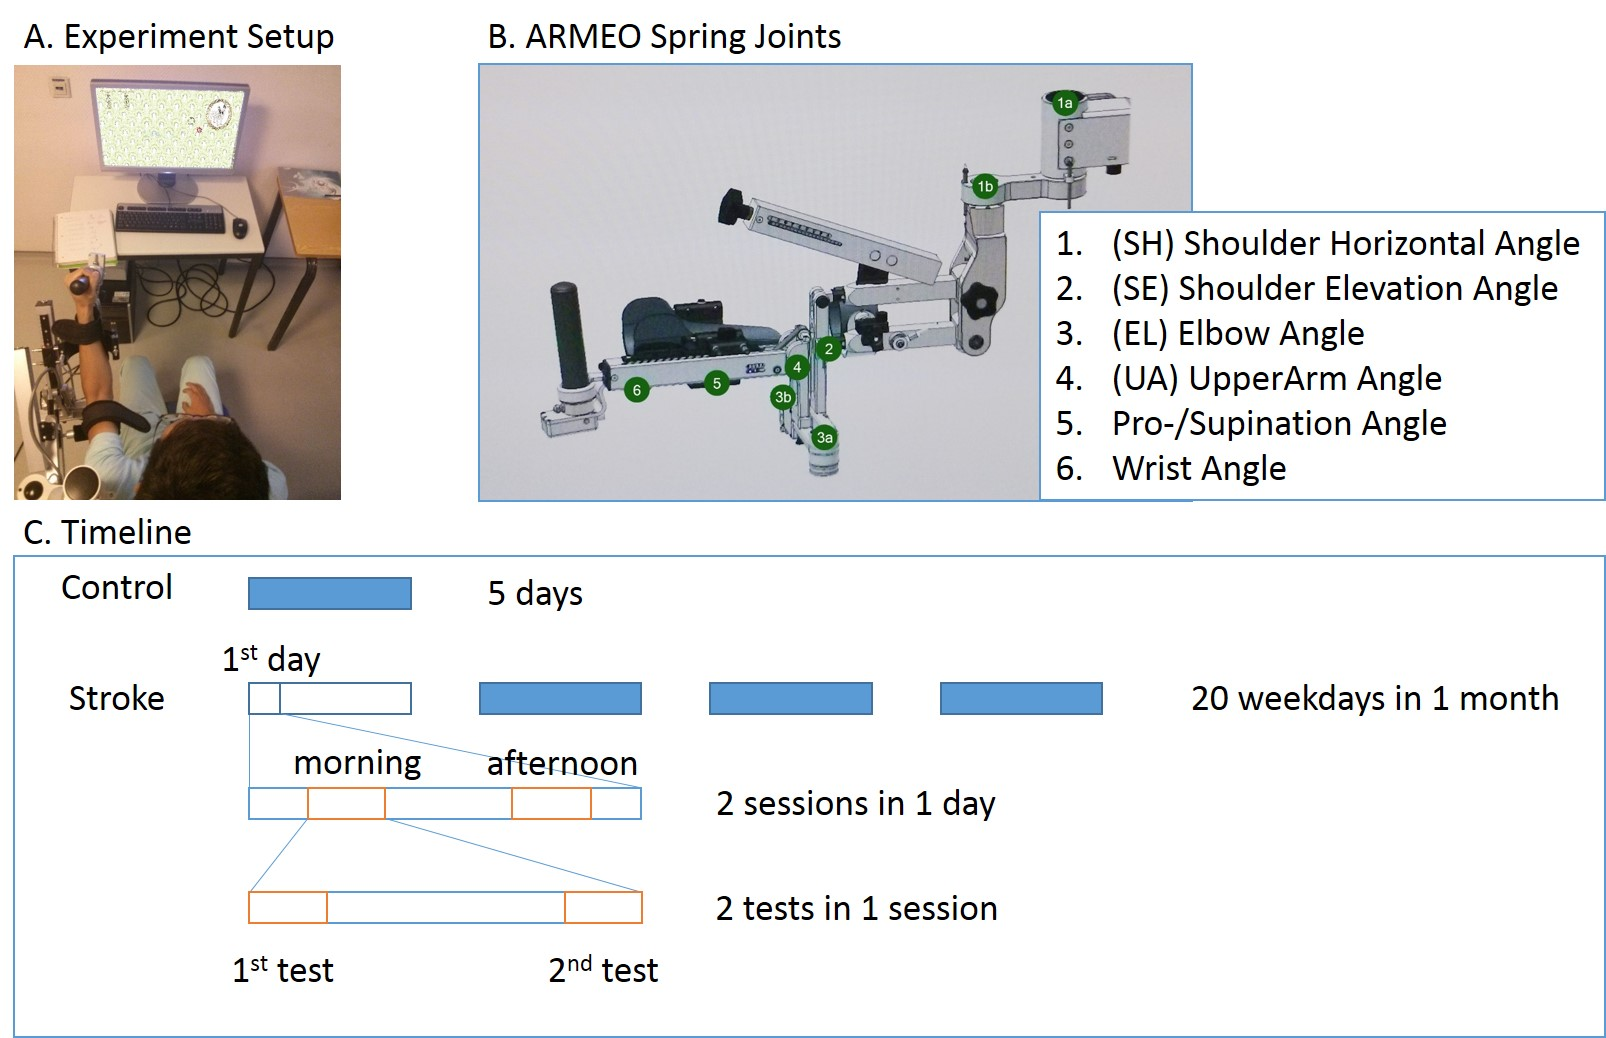
\includegraphics[width=1\linewidth]{figures/1setup&schedule}
	\caption[Methods.]
	{Methods.
		A. Experiment setup: Participants sat in front of a vertical screen on which the video games were displayed. In the ladybug test given at the beginning and end of each training session, the cursor responded to vertical movements of the end-effector. 
		B. ARMEO Spring device: Joints of ARMEO Spring. Summation of joints 1a and 1b gives the Shoulder Horizontal (SH) angle, joint 2 the Shoulder Elevation (SE) angle, joint 3a (for the right arm) and 3b (for the left arm) the elbow (EL) angle, joint 4 the ForeArm (FA) angle, joint 5 pronation and supination angle, and joint 6 the wrist angle. 
		C. Training and testing schedule: each day, a session was administered in the morning and a second in the afternoon. Ladybug tests was administered at beginning and end of each training session. The Control group received 5 consecutive days training, whereas the stroke group received 20 consecutive weekdays training.}
	\label{fig:1setupschedule}
\end{figure}

\subsection{Data Analysis}

\textbf{Preprocessing.}
We filtered the data with a second order Butterworth filter \cite{Butterworth1930} with a cutoff frequency of 5 Hz. 
We defined a trial as the movement between two consecutive targets. 
A trial was considered successful if it started from previously caught target and led to the catching of next target. 
Only successful trials, that is, trials in which the participant caught the next ladybug within the pre-specified time of 10 sec (control 99.8\%, stroke 78.2\%) were included in the analysis. 
We excluded tests in which participants caught less than 25\% of the ladybugs (0.7\% of all tests in stroke group, 0\% in control group).

\textbf{Task Space Performance.}
We characterized task space performance in a test via the average number of peaks in the velocity profiles. 
This measure of movement smoothness has been used to quantify movement smoothness in non-disabled subjects \cite{Brooks1973} and individual post-stroke. 
The number of peaks in the velocity profile have been shown to decrease following robotic training post-stroke.  
To calculate the number of peaks in each movement, we computed the derivative of velocity (tangential acceleration) and counted the number of times it went from positive to negative. 
We then took the average of number of peaks ($ p $) of all successful trials in the test. 

\textbf{Mixed Effect Models of Learning and Recovery}

Stroke is characterized by high variability in lesion, impairment, spontaneous recovery, and responsiveness to therapy \cite{Cramer2008}. 
We have previously shown that including mixed-effects in non-linear models can account for between-individual differences in performance and changes of performances during motor training post-stroke \cite{Park2017}. 
Here, similarly, we therefore used non-linear mixed effects to precisely account for differences in baseline performance, as well as learning and recovery for each participant. 

Specifically, we modeled the dynamics of average number of peaks $ p $ in the velocity profiles in each test as exponential functions of time $ t $ represented by task number, with mixed effects \cite{Lindstrom1990}. 
Because visual observation seemed to indicate that changes in the average number of peak decreased according to a single exponential-like decay for participants in the control group, we considered a model with a single exponential formulation
\begin{equation}\label{eqn:singleexp}
p_{i,j} = A_i \exp(-B_i t_{j}) + 1 + \epsilon_{i,j}
\end{equation}
where $ t_{j} = j $ is the test number $ j $, 
$ A_i $ is the mixed-effect coefficient representing the amplitude of the exponential for participant $ i $,
$ B_i $ is the mixed-effect coefficient representing the learning rate,
and $ \epsilon_{i,j} $ is the residual. 
We choose an asymptote of 1 because it is the theoretical limit of number of peaks in velocity profiles.
Note that we verified that a model with two exponentials did not better fit the data that a model with a single exponential for this group, based on the Bayesian Information Criterion. 
We also verified that a model with random effects on both the amplitude and the learning rate better fit the data than a model with only fixed effects. 

Because visual observation seemed to indicate that changes in number of peaks over 4 weeks of training was initially fast and then slower for the participants in the stroke group, we considered a model with two exponential components 
\begin{equation}\label{eqn:doubleexp}
p_{i,j} = A^f_{i} \exp(-B^f_{i} t_j) + A^s_{i} \exp(-B^s_{i} t_j) + 1 + \epsilon_{i,j}
\end{equation}
where $ A^f, A^s, B^f $ and $ B^s $ are constraint to be positive, and $ B^f > B^s $, therefore the first term stands for a fast component, the second a slow component. 
Note that we verified that a model with two exponentials better fit the data than a model with a single exponential for this group, based on the Bayesian Information Criterion. 
We also verified that a model with random effects on the amplitudes and the learning rates for both components better fit the data than a model with only fixed effects. 
The models were all fit with the function \textsf{nlmefit} in Matlab 2016a.

%\textbf{Conversion of Joint Angles}
%The recordings from ARMEO Spring are joint angles of the exoskeleton, different from anatomical joint angles.
%It is therefore important to infer anatomical joint angles from exoskeleton joint angles. 

\textbf{Synergy Extraction and Analysis}

We use Principal Component Analysis (PCA) to extract joint synergies from each ladybug test.
The principal components of joint angles, which captures most of the variance presented in the data, can be interpreted as joint synergies and has been previously used in both non-disabled and stroke individuals \cite{Soechting1997}. 
As a dimension reduction method, PCA provides components that explain the most variability in joint angle space. 
Here, because the last two joints (pronation/supination and wrist angle) accounted for only 12.4\% of the variance in the control group, and 4.6\% in the stroke group, we ignored these joints in the synergy analysis.  
Similarities between groups of synergies can be measured via the principal angle between two subspaces \cite{Bockemuehl2010}, which is the minimum rotation angle required to rotate one subspace onto the other \cite{Bjoerck1973}. 
A principal angle of $ \ang{0} $ indicates identical synergy patterns, whereas $ \ang{90} $ indicates maximal differences.  
For each stroke participant, we computed the principal angle $ \phi $ between his/her synergies from every test and the average synergies of the non-disabled participants computed with the data from the last 4 tests, in the last day of training. 
At this point, performance in this group was near asymptote (see below); we thus assumed that synergies computed at this time formed a basis for comparison of the synergies in the stroke group. 

$ \phi(t) $ ($ t $ for test) reflects the abnormality of participant’s joint synergy patterns throughout training. 
Because we hypothesized that initial movement abnormality would slow down recovery, and to minimize variability, we fitted a linear mixed effect model to $ \phi(t) $ with a fixed effect on the intercept $ \phi(0) $ and   a random effect on both the intercept and slope (the we didn’t include fixed effect on the slope because it was not significant when included in the model)  using the first 10 tests  . 
To investigate how joint synergies affects task space learning, we correlated the initial abnormal synergy index, $ \phi(0) $, with the (fast and slow) learning rates. 

%
%PCA belongs to a family of Dimension Reduction methods.
%Principal Components of joint angles, which captures most of the variance presented in the data, can be interpreted as joint synergies.% \cite{}.
%In this study, we only look at the first two synergies which on average account for 83.9\% joint angle variance for control group, 83.1\% for stroke group.
%Joint synergies of healthy participants are quite stable across individuals.
%We calculate the averaged synergies shown in figure \ref{fig:6synergy}C.
%
%To evaluate the synergy pattern of stroke participant, we use the principal angle %\cite{}
%between subspaces that are spanned by synergies.% \cite{}.
%Generally, the principal angle $ \phi $ between two subspaces is the minimum rotation angle required to rotate one subspace onto the other.
%A principal angle of \ang{0} indicates the same synergy patterns, whereas \ang{90} indicates completely different ones.
%Therefore we refer to this angle as synergy abnormality.
%We use Matlab 2016a \textsf{subspace} %\cite{}
%to calculate the principal angle. 
%
%For each stroke participant, we investigate the synergy abnormality (principal angle) $ \phi $ between his synergies from every test and the average healthy synergies.
%$ \phi(t) $ ($ t $ for test) reflects the abnormality of participant's joint synergy patterns throughout training. 
%We fit a linear mixed effect model to $ \phi(t) $ with a fixed effect on the intercept $ \phi(0) $ and a random effect on both the intercept and slope (we do not include a fixed effect on the slope because it is not significant when included in the model).
%%The intercept $ \phi(0) $ tells us how different this participant's synergy pattern is initially different from the control group.
%%It is therefore a measure of joint coordination prior training.
%
%To investigate how joint synergies affects task space learning, we correlate $ \phi(0) $ with task space (fast and slow) learning rate.


\textbf{Joint Space Variability}

We adapted the method from \cite{Singh2016} to quantify joint space variability and its relevance to the task space. 
Because data from the reaching tests in the present study were collected during the ladybug test provided by Hocoma, there are two main difference between the tests used in the present study and those of \cite{Singh2016} however. 
The first is that, whereas the tests in \cite{Singh2016} contains multiple repetition of the same movements, the ladybug tests contain a single movement for each target. 
Thus, it is not possible to compute variability within a single ladybug test. 
We therefore used data from multiple consecutive tests. 
Second, whereas the variability was calculated at baseline, that is, before the perturbation was introduced in the \cite{Singh2016} study, we do not have access to reaching data without gravity support before training (without such gravity support, it is probable that a number of individuals post-stroke would not be able to perform the test). 
We therefore  computed the task-irrelevant variability from the last 10 consecutive tests. 
We used the last 10 tests because our initial inspection of the data and double exponential models (see results) showed that changes in average number of peaks in the last 10 tests were small, because fast changes due to learning had vanished. 
In addition, whereas \cite{Singh2016} computed variability at the time of maximum velocity, we computed task-irrelevant variability when the cursor entered the target area because of very large between- and within-subject variability in task-space at the time of maximum velocity.
Note that for this analysis, we again ignored the two wrist joints because of small variance. 

Here, we briefly describe the method, adapted from \cite{Singh2016}.
The nonlinear forward kinematics model of the exoskeleton is given by
	\begin{equation}\label{eqn:nonlinearForwardKinematics}
		\bm{r} = f(\bm{\theta})
	\end{equation}
where $ \bm{r} = (x,y)^T $ is the location of the end effector, $ \bm{\theta} $ is joint angles (see Table \ref{tab:devicedof} and Figure \ref{fig:1setupschedule}B for details). 

The mean joint configuration across the last 10 tests at one specific ladybug ($ b $) is denoted by $ \bar{\bm{\theta}}_b $.
We will omit index $ b $ for convenience.
The Jacobian matrix at configuration $ \bar{\bm{\theta}} $ is obtained through forward kinematics (Eqn. \ref{eqn:nonlinearForwardKinematics})
	\begin{equation}
		\bm{J}(\bar{\bm{\theta}}) = \frac{\partial f(\bm{\theta})}{\partial \bm{\theta}} \Big\rvert_{\bar{\bm{\theta}}}
	\end{equation}
which is a 2 by 4 matrix.
The null space of Jacobian $ \bm{J} $ can be represented by basis of the space $ \bm{\xi}_i $, $ i= 1,2 $ which satisfy
	\begin{equation}
	\bm{J}(\bar{\bm{\theta}}) \bm{\xi}_i = 0
	\end{equation}
Because movements in the null space ($ \bm{\xi}_i $) have no effect on the location of end effector, hence is task irrelevant (we therefore call the null space as the task-irrelevant space).
For a specific test ($ t $) , the deviation of joint angles from $ \bar{\bm{\theta}} $ is
	\begin{equation}
	\Delta\bm{\theta}_t = \bm{\theta}_t - \bar{\bm{\theta}}
	\end{equation}
Omitting the index $ t $, the projection of $ \Delta\bm{\theta} $ to the task-irrelevant space is
	\begin{equation}
	\Delta\bm{\theta}_{\text{null}} = \sum_i^m \langle \Delta\bm{\theta}, \bm{\xi}_i \rangle \bm{\xi}_i, m=2
	\end{equation}
where $ \langle,\rangle $ represents inner product.
In the end, we quantify the task-irrelevant variability by calculating the mean of squared $ \Delta\bm{\theta}_{\text{null}} $
	\begin{equation}\label{eqn:nullvar}
	V_{\text{null}}(t,b) = \mathbb{E}_{t,b} (\Delta\bm{\theta}_{\text{null}}^T\Delta\bm{\theta}_{\text{null}})
	\end{equation}
where $ t,b $ index tests and targets (ladybugs). 
We then average $ V_{\text{null}}(t,b) $ across tests ($ t $) and targets ($ b $) as the measure of task-irrelevant variability of a participant. 
Because $ V_{\text{null}} $ is similar to the calculation of variance, it has unit of $ \text{deg}^2 $.
It is on average the summation of variance across all joints.

To obtain variability in the orthogonal (task-relevant) space, we simply replace $ \bm{\xi}_i $ with the basis of the orthogonal space, $ \bm{\psi}_i $, $ i= 1,2 $  :
	\begin{equation}
	\Delta\bm{\theta}_{\text{orth}} = \sum_i^m \langle \Delta\bm{\theta}, \bm{\psi}_i \rangle \bm{\psi}_i, m=2
	\end{equation}
and the task-relevant space variability is
	\begin{equation}\label{eqn:taskvar}
	V_{\text{orth}}(t,b) = \mathbb{E}_{t,b} (\Delta\bm{\theta}_{\text{orth}}^T\Delta\bm{\theta}_{\text{orth}})
	\end{equation}
Finally, note that this kinematic model (Eqn. \ref{eqn:nonlinearForwardKinematics}) was provided to us by Hocoma, the ARMEO Company. 

\textbf{Linear Regression.}
When performing linear regression between variables, we identified outliers through Cook’s Distance \cite{Cook1977}. 
The Cook’s Distances of outliers are greater than $ 4/n $, where $ n $ is the number of data points. 
When outliers were detected, we performed a robust regression method with the bisquare weight function \cite{Hoaglin1983}. 
We verified in all regression analyses that test difficulty was not significant when included as a covariate. 
Our predefined threshold for statistical significance was 0.05. 
All analyses were performed in Matlab.
%In this study, when doing linear regression, we identify outliers through Cook's Distance (Cook, 1977).
%Cook's Distance $ D $ uses a data point's residual and leverage \cite{Chatterjee1986} to estimate the influence of a data point on least-square regression.
%We label data point $ i $ as an outlier if $ D_i > 4/n $ ($ n $ is the number of observations) (Bollen, 1985). %\cite{Bollen1985}.
%Instead of removing them, we adopt robust regression method with the bisquare weight function (Hoaglin, Mosteller, 1983).

\outline{2}{Results}
\section{Results}

Stroke participants performed an average of 74 $\pm$ 13 tests, with range of 33 to 86 tests. 
36\% performed the 80 tests. 
All control participants performed the 20 tests.

Participants typically showed large changes in performance during the duration of training. 
Figure \ref{fig:2stroketrajexamp} shows representative trajectories in both task space and joint space for a participant posts-stroke (UEFM pre = 39, post = 63). 
After training, the trajectories in task space are straighter, and the joint trajectories seem smoother.

\begin{figure}
	\centering
	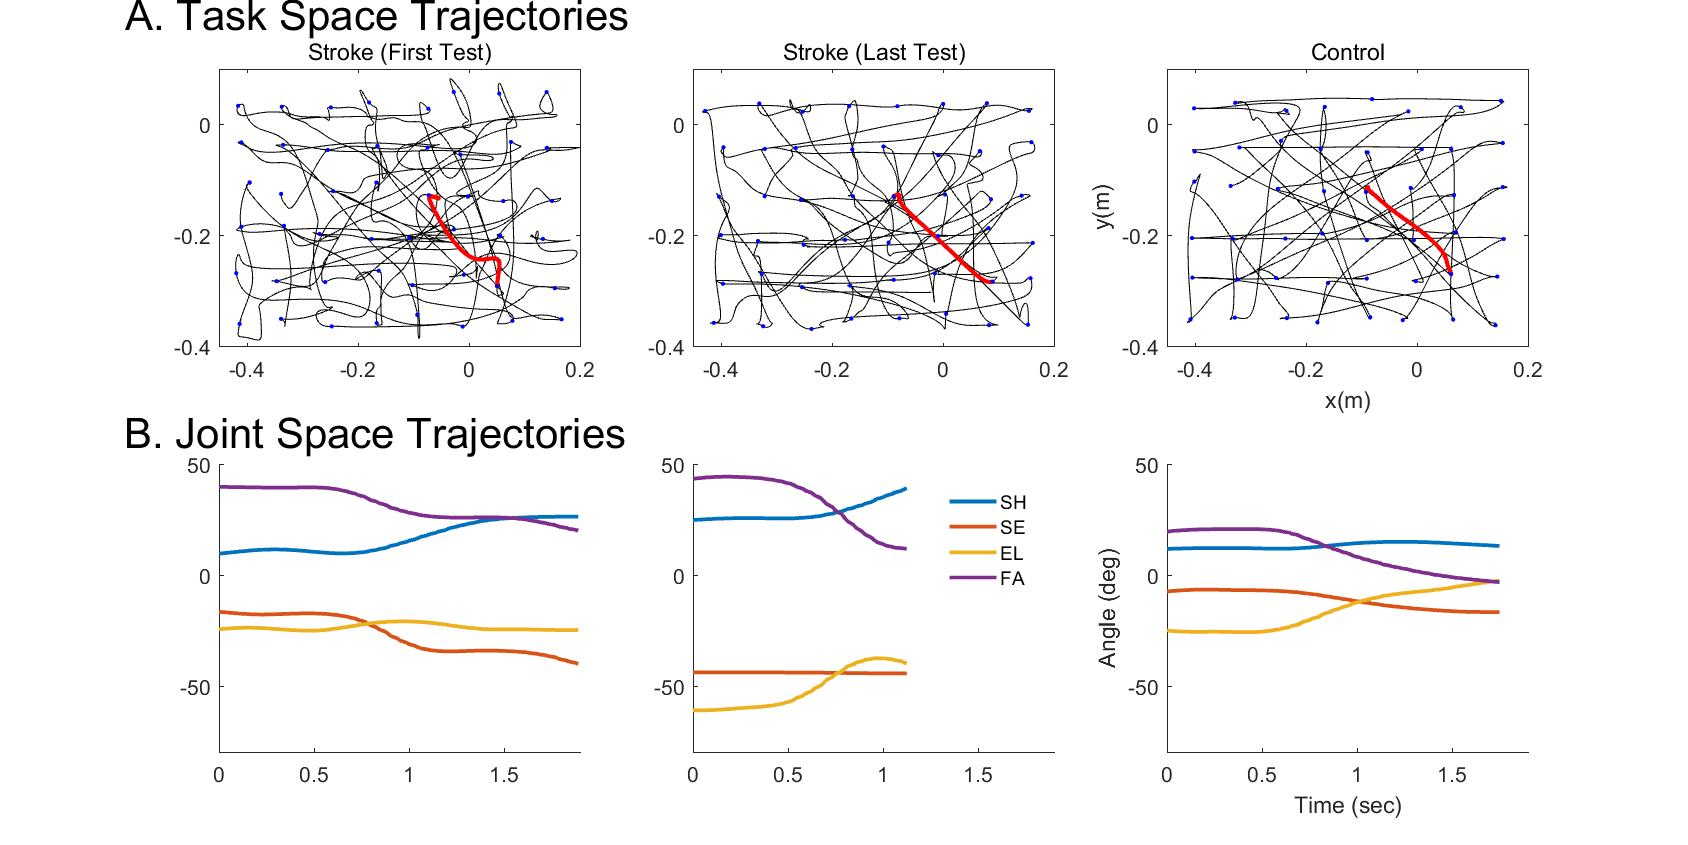
\includegraphics[width=1\linewidth]{figures/2strokeTrajExamp}
	\caption[Representative trajectories]
	{Representative trajectories. 
		A. Representative task space trajectories. Trajectories after training are straighter.
		B. Representative joint space trajectories, correspond to the red part trajectories in panel A, moving from the center to bottom right. Only the first four ARMEO joints are shown.}
	\label{fig:2stroketrajexamp}
\end{figure}

\subsection{Task Space Performance}

Figure \ref{fig:3nopfixran} shows the average number of peaks in each test modeled by exponential functions. 
Stroke participants show large improvements in the number of peaks, with a decrease of approximately three peaks on average over the course of training (Figure \ref{fig:3nopfixran}B). 
However, control subjects exhibit fewer number of peaks on average, even before training (Figure \ref{fig:3nopfixran}A).

For the stroke group, the mixed effect double exponential model better fits the data than linear or single exponential models or models without mixed effects (lowest BIC: Bayesian Information Criteria, which balances fitting errors and number of parameters). 
For subjects in the control group, a single exponential model has a smaller BIC than a double exponential model.

\begin{figure}
	\centering
	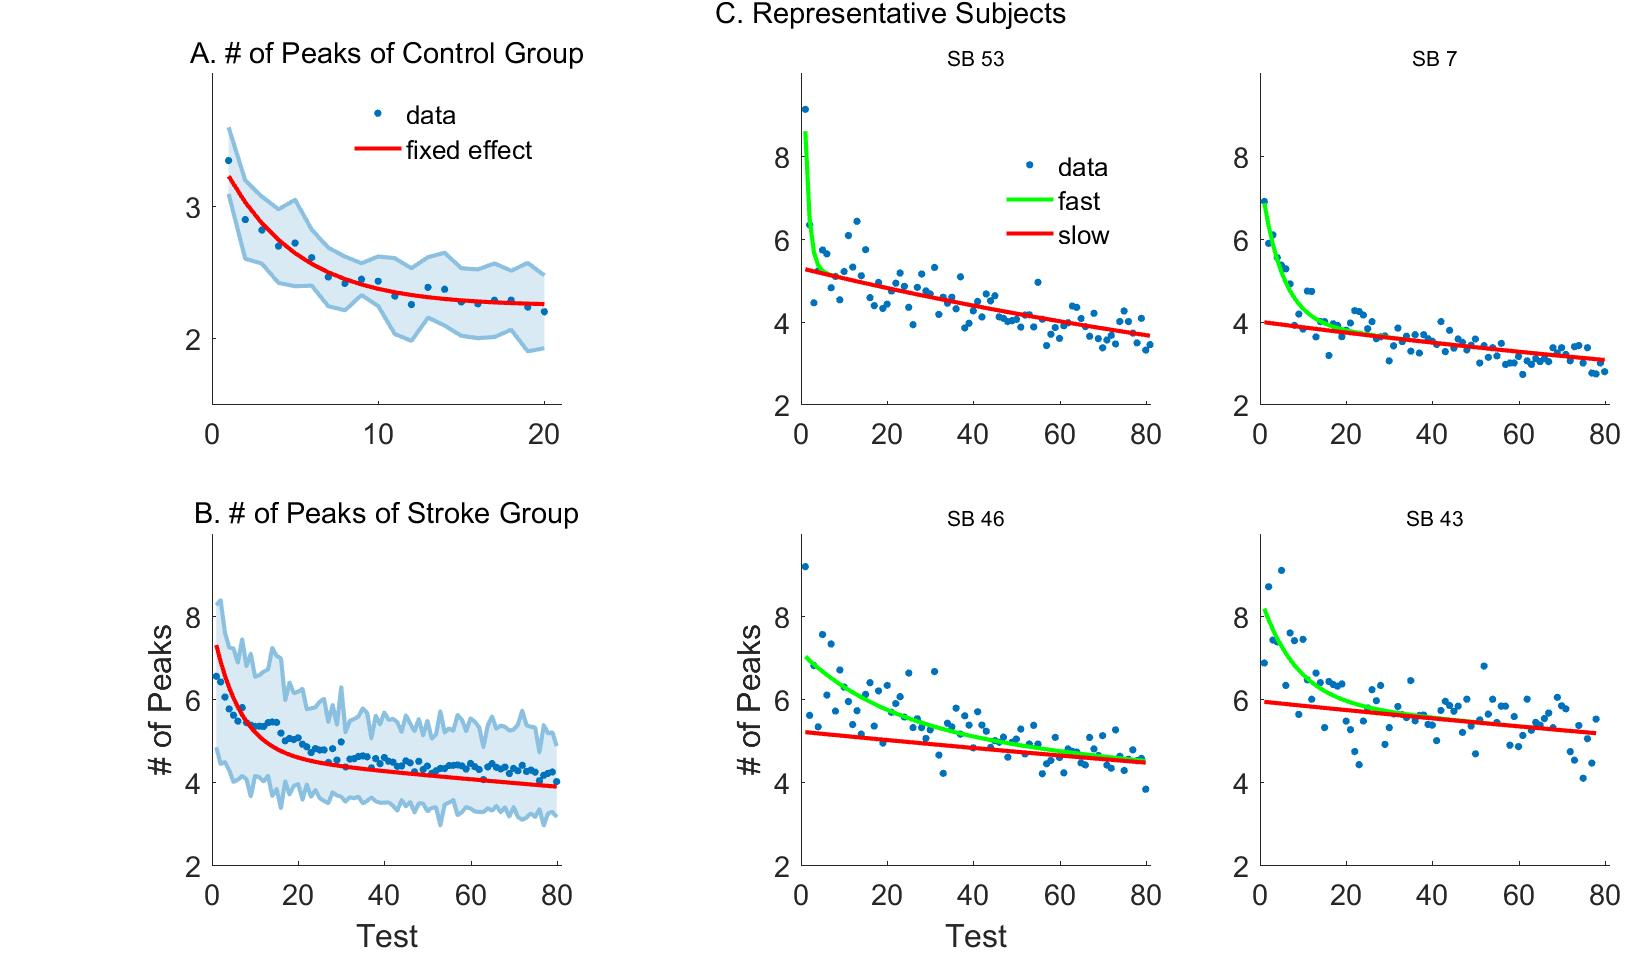
\includegraphics[width=1\linewidth]{figures/3nopFixRan}
	\caption[Double Exponential Model]
	{Double exponential model of the average number of peaks in velocity profile in each ladybug test. 
		A,B: Group average (blue dots) and fixed effects (red line) of the fitted exponential model of number of peaks for the control (A) and stroke groups (B). Shaded area represents standard deviation (note the different scale for both axes in both groups); 
		C: Representative participants. 
		SB 53: fast learning rate and large task-irrelevant variability; 
		SB 46: slow learning rate and small task-irrelevant variability (see Figure \ref{fig:5learnratevsnullvar} for task-irrelevant variability);
		SB 7: fast recovery rate and small initial synergy abnormality;
		SB 43: slow recovery rate and large initial synergy abnormality (see Figure \ref{fig:6synergy} for initial synergy abnormality).
	}
	\label{fig:3nopfixran}
\end{figure}

The double exponential mixed effect model of the stroke groups (Equation \ref{eqn:doubleexp}) tields two learning rates $ B^f $ and $ B^s $. 
We refer the smaller of the two, $ B^s $ as the slow learning rate, the larger, $ B^f $ the fast learning rate.
Figure \ref{fig:3nopfixran}C shows examples of individual fitting.
The slow component, due to small learning rate, is approximately linear; but the fast component usually reaches asymptote during the training.
For the stroke group, the fast learning rate corresponds to a time constant of 13 $\pm$ 19 tests; and the slow learning rate with a time constant of 352 $\pm$ 123 tests (see Figure \ref{fig:3nopfixran}). 
For the control group, the time constant is 4.4 + 1.6 tests (as a reminder, there were 4 tests per day, but training and testing was only performed on weekdays). 

The number of peaks at test 80 predicted by the mixed effect model average number of peaks post training and UEFM post training are significantly correlated (least square regression: p = 0.0003; robust regression p = 0.0009; Figure \ref{fig:4slowcomponentisrecovery}A).
Note however that the pre-training UEFM does not correlate with the number of peaks on the first test 1 predicted by the model (p = 0.10).
In addition, the change in number of peaks before and after training from test 1 to test 80 due to the slow process (term $ A_i^s \exp(-B_i^s t_j) $) in Equation \ref{eqn:doubleexp}), correlates significantly (both least square and robust regression: p $<$ 0.0001) with the change of UEFM (Figure \ref{fig:4slowcomponentisrecovery}B). 
In contrast, the change in number of peaks before and after training due to the fast process does not correlates (p = 0.33) with the change of UEFM. 
This indicates that the slow learning process, rather than the fast one, reflects a recovery of arm movements. 
The fast process therefore reflects change in arm movements due to motor learning. 
We therefore refer to $ B^s $ as the recovery rate, and $ B^f $ as the learning rate.

\begin{figure}
	\centering
	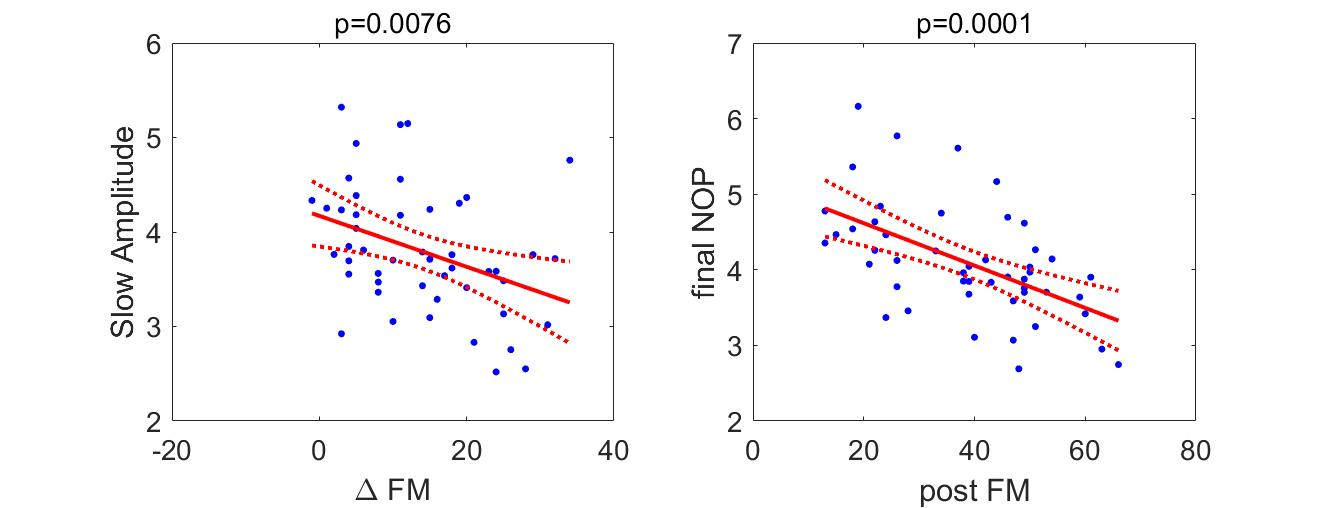
\includegraphics[width=1\linewidth]{figures/4slowComponentIsRecovery}
	\caption[Slow component corresponds to recovery as meaured by the changes of UEFM]
	{Slow component corresponds to recovery as meaured by the changes of UEFM.
		A: The number of peaks post training correlates with UEFM post training;
		B: The change of number of peaks due to the slow process correlates with the change of UEFM, prior and post training.
	}
	\label{fig:4slowcomponentisrecovery}
\end{figure}

\subsection{Synergy Analysis}

The first two synergies account on average for 83.9\% joint angle variance for control group, 83.1\% for stroke group. 
We calculated the averaged synergies (see Methods; Figure \ref{fig:6synergy}C) as a basis for comparison with the stroke synergies. 
The first average synergy is composed of Shoulder Horizontal (SH) rotation and Elbow (EL) angle, and it is responsible for horizontal movements. 
The second synergy is composed of Shoulder Elevation (SE) angle and Forearm (FA) angle, and it is responsible for vertical movements. 
Synergies for the stroke participants show large between-participant differences. 
They can share a similar structure as the control group (Figure \ref{fig:6synergy}B), or have different structure (Figure \ref{fig:6synergy}A).

The initial synergy abnormality index correlates with the recovery rate $ B^s $ (see Equation. \ref{eqn:doubleexp}) as shown in Figure \ref{fig:6synergy}D (least square regression: p = 0.0048; robust regression p = 0.0114), indicating that patients with large synergy abnormality index recovers more slowly (such as SB 43, see Figure \ref{fig:3nopfixran}C) than participants with small abnormality (such as SB 7, see Figure \ref{fig:3nopfixran}C).

\begin{figure}
	\centering
	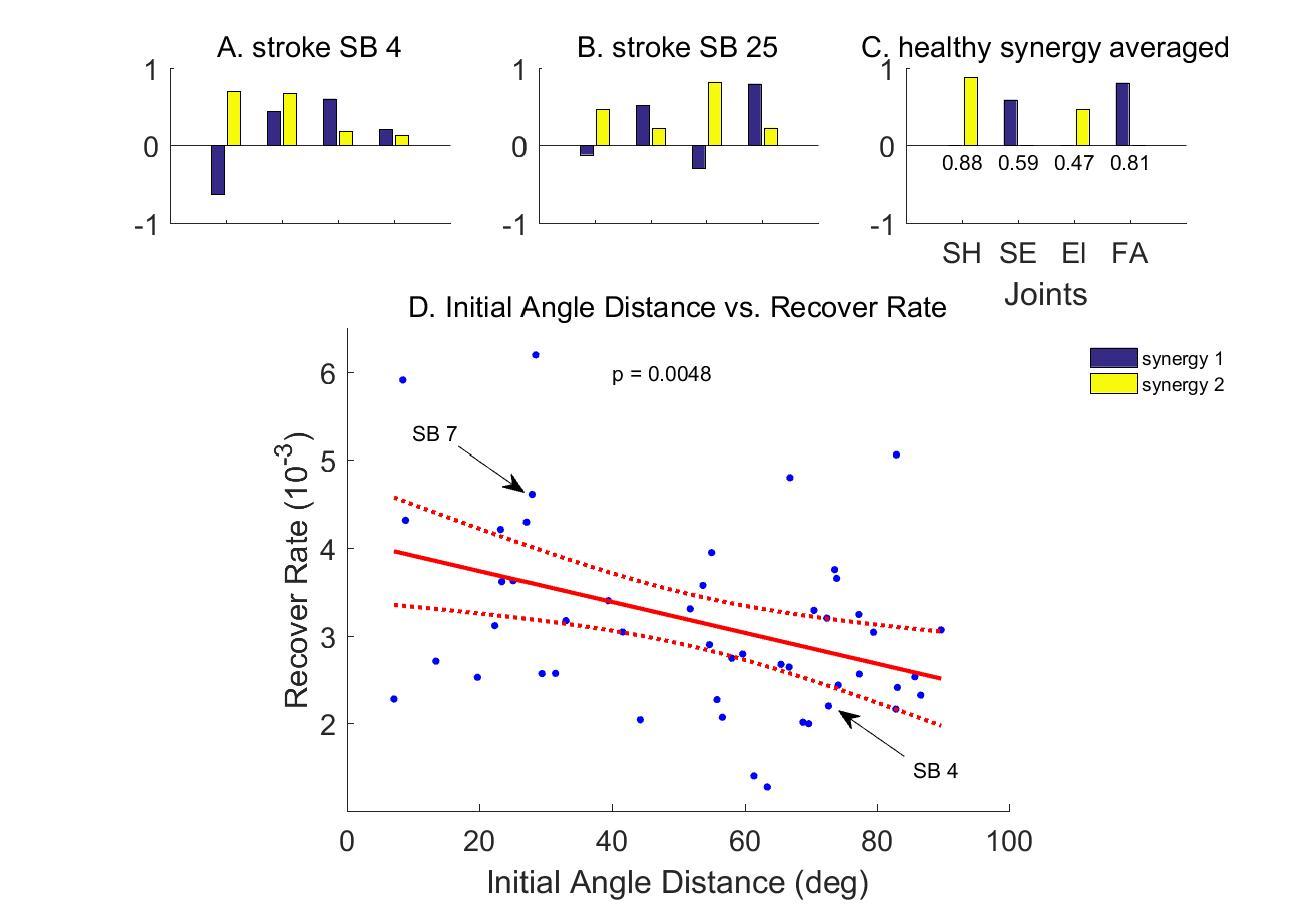
\includegraphics[width=1\linewidth]{figures/6synergy}
	\caption[Synergy Analysis]
	{Synergy Abnormality hinders recovery. 
		A,B. Radar plot of synergies as uncovered with a PCA analysis. Blue and red lines show the first and second synergies. Dashed black line indicates zero.
		A. Representative participant with abnormal synergies and normal synergies;
		B. Averaged synergies of participants in the control group;
		C. Initial synergy abnormality reduces recovery rate. SB 7 and 43 are representative participants, whose initial synergy patterns are shown in panel A and B, learning curves are shown in panel D; 
		D. Learning curves of representative subjects 7 and 43.}
	\label{fig:6synergy}
\end{figure}

\subsection{Joint Space Variability}

Both the control and stroke groups display much larger task-irrelevant variability than task-relevant variability.
For the stroke group, the task-irrelevant variability is on average $\ang{18.3} \pm \ang{19.4} $ (measured by standard deviation,$ \sqrt{V_\text{null}} $); whereas the task-relevant variability ($ \sqrt{V_\text{orth}} $) on average is $\ang{3.1} \pm \ang{2.9} $.
For the control group, the task-irrelevant variability is $ \ang{18.3} \pm \ang{13.8} $, whereas the task-relevant variability is $ \ang{2.2} \pm \ang{1.5} $.

For the stroke group, rask-irrelevant variability positively correlates with the learning rate $ B_f $, as shown in Figure \ref{fig:5learnratevsnullvar} (least square regression p $<$ 0.0001; robust regression p = 0.0016). 
Participants with small task-irrelevant variability learn slower (such as SB 46, see Figure \ref{fig:3nopfixran}C: SB 46);
participants with large task-irrelevant variability learn faster (such as SB 46, see Figure \ref{fig:3nopfixran}C: SB 53).
There was no correlation between task-irrelevant variability and learning rate for the control group (p = 0.2170).

\begin{figure}
	\centering
	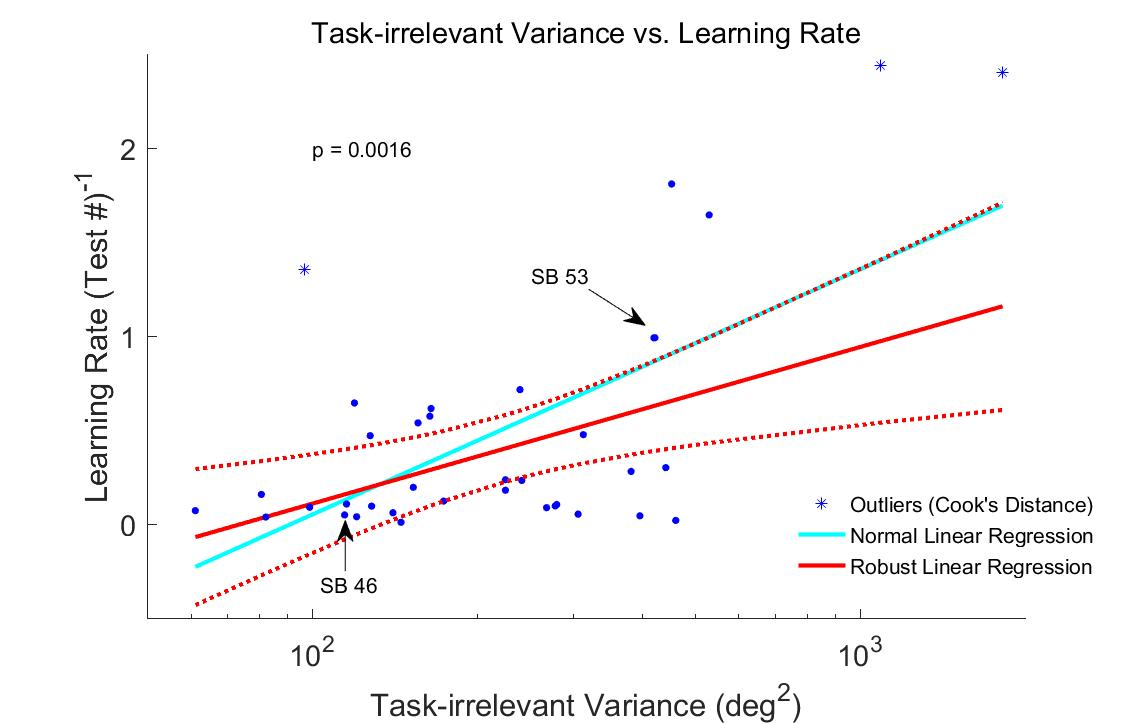
\includegraphics[width=1\linewidth]{figures/5learnRateVSnullVar}
	\caption[Exploration of Joint Redundancy facilitates learning]
	{Exploration of Joint Redundancy facilitates learning. 
		A. The learning rate of the double exponential model correlates with the (log of) null space variability. 
		B. Learning curves of representative subjects SB 53 and 46. }
	\label{fig:5learnratevsnullvar}
\end{figure}



\outline{2}{Discussion}
\section{Discussion}
We characterize kinematics performance with a double exponential model of number of peaks, and show evidence that the two components link to motor learning and recovery respectively. 
The mixed effect estimation of parameters allow us to obtain estimations of individual learning rates.

Task-irrelevant variability, or variance in the UnControlled Manifold (UCM), is a source of variability that doesn’t affect the execution of a task, which can be represented by variables. 
In the original study, \cite{Scholz1999} demonstrated that during a functional task, certain relevant variables are not controlled.
The redundancy of human arm kinematics dictates that there must be task-irrelevant variability (the variability that does not affect endpoint trajectories) in the joint space. 
We measure this task-irrelevant variability with adapted method from \cite{Singh2016}. 
Although this variability is task irrelevant, it is not unnecessary since it brings flexibility and allow versatile joint coordination for some specific task. 
However, how task-irrelevant variability affects learning (in healthy subjects) or recovery (in stroke survivors) is a question worth investigating. 
\cite{Singh2016} suggested that this variability, as a form of redundancy exploitation, helps motor adaptation and learning. 
In our study, we found a correlation between task-irrelevant variability and learning rate of post-stroke individuals, suggesting that it also helps stroke individuals to learn a novel task.

Joint synergies are extracted through Principal Component Analysis (PCA). 
As a dimension reduction method, PCA provides components that explain the most variability in joint angle space. 
Along with other dimension reduction methods, PCA has been used to extract joint synergies \cite{Kordelaar2012}. 
Similarities between synergies can be measured through the angle between two synergies in joint angle space, and similarities between groups of synergies can be measured through the angle between two subspaces \cite{Bockemuehl2010}. 
We couldn't verify the method used in \cite{Bockemuehl2010}, instead we use numerical method in \cite{Bjoerck1973} to calculate angles between subspaces. 
A correlation between joint synergy abnormality and recovery rate may suggest that joint coordination patterns are important for functional recovery.

